\begin{figure*}[h]
        \begin{subfigure}{.66\columnwidth}
            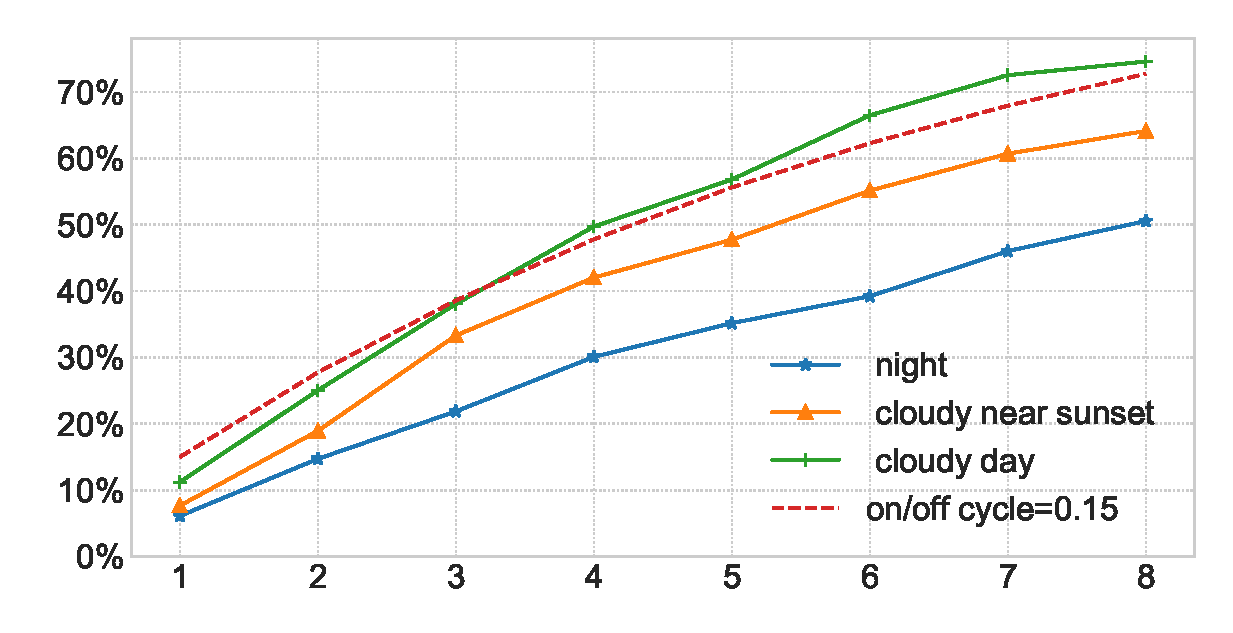
\includegraphics[width=\textwidth]{figures/sysAvailability}
                \caption{The \cis is powered by uncontrollable light sources---artificial light (night) and sunlight (day).}
            \label{fig:solarPwrCIS}
        \end{subfigure}\hfill
        \begin{subfigure}{.66\columnwidth}
            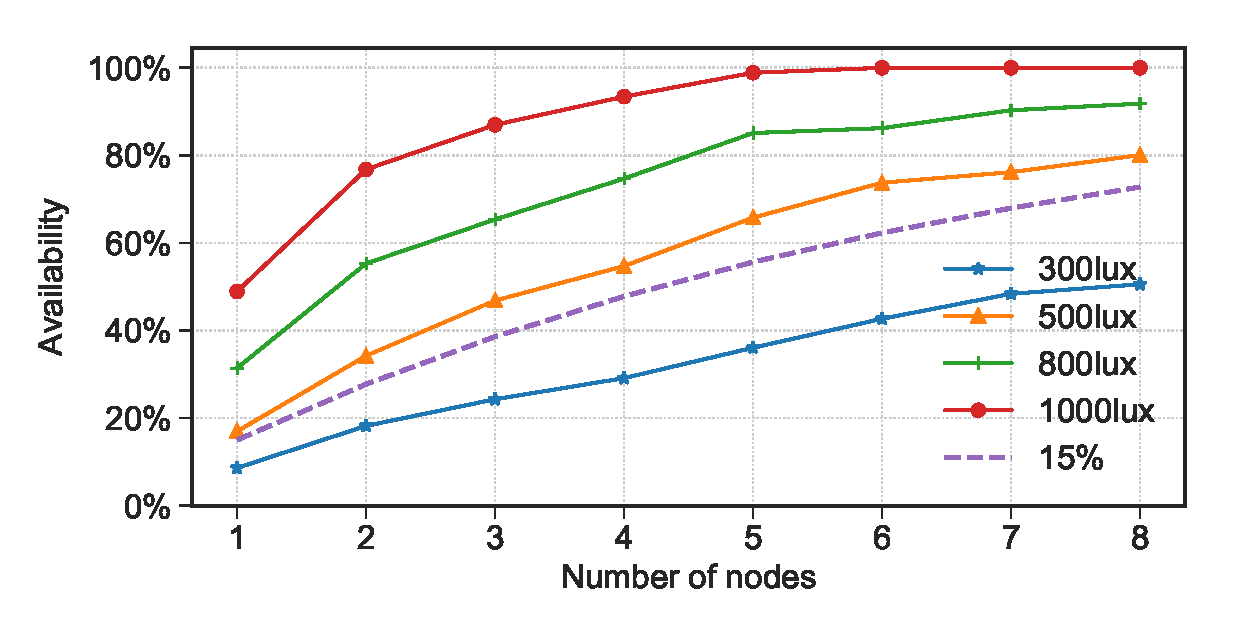
\includegraphics[width=\textwidth]{figures/sysAvailability_artificial-light}
                \caption{The \cis is powered by a controllable array of LEDs. \vspace{1em}}
            \label{fig:artPwrCIS}
        \end{subfigure}\hfill
        \begin{subfigure}{.66\columnwidth}
            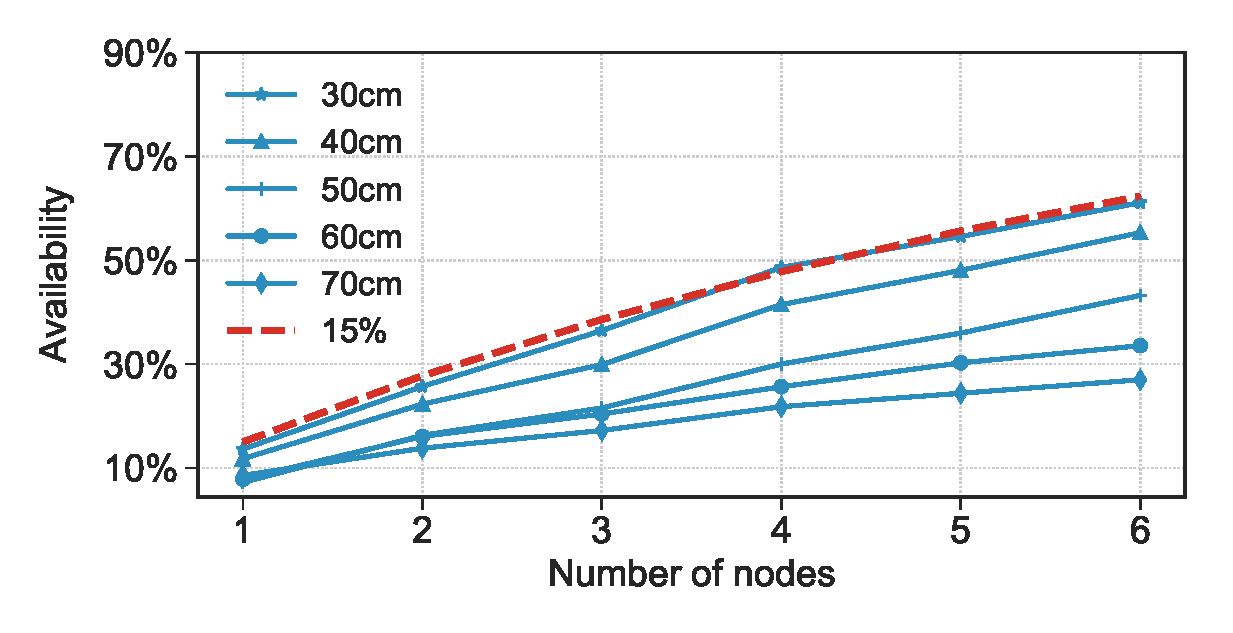
\includegraphics[width=\textwidth]{figures/rf_sysAvailability}
                \caption{The \cis is powered by an RF reader~\cite{r420_website} located 30-70\,cm away from the RF tags (WISPs~\cite{smith2006wirelessly}).}
            \label{fig:rfPwrCIS}
        \end{subfigure}
        \caption{The \fullcis's availability for differed numbers of intermittent nodes and energy sources. 
        The modeled availability---represented by the dashed lines when the average node duty cycle is 15\%---approximates the measured availability with high accuracy.}
        \label{fig:pwrCIS}
\end{figure*} 
To evaluate the performance (availability) of the \fullcis, we conducted several experiments in different energy conditions and with different event arrivals patterns. 
%
\subsection{Availability}
%%%%%%%%%% ToDo %%%%%%%%%%
% Experiment setup
Irrespective of the energy source (RF or light) we showed in Figure~\ref{fig:power_cycles} that the power cycles of a \cis's nodes are different, which leads to a uniform distribution of their on-times, as we argued in Section~\ref{subSec:availability}. We captured the expected joined availability of these nodes in Model~\ref{eq:cisModel}.  Here, we validate model by comparing the modeled availability of a \cis against data captured with different hardware (solar- and RF-powered nodes) in different scenarios.
% the measured ones under different powering conditions and with different hardware. 
 
Figure~\ref{fig:pwrCIS} shows the availability of three \cis{}s when they are powered by sunlight, artificial light, and RF and for a different number of intermittent nodes.
%%%%%%%%%% ToDo %%%%%%%%%%
% clarify that the RF and solar power nodes use different hardware.
The results clearly confirm our expectation: when the power cycles are slightly different, the on-times are uniformly distributed. The results also validate our model; the dashed lines represent the modeled availability when the nodes duty cycle is 15\%.

\subsubsection{Availability on a Fine Scale}
%
\begin{figure}[t]
    \centering
     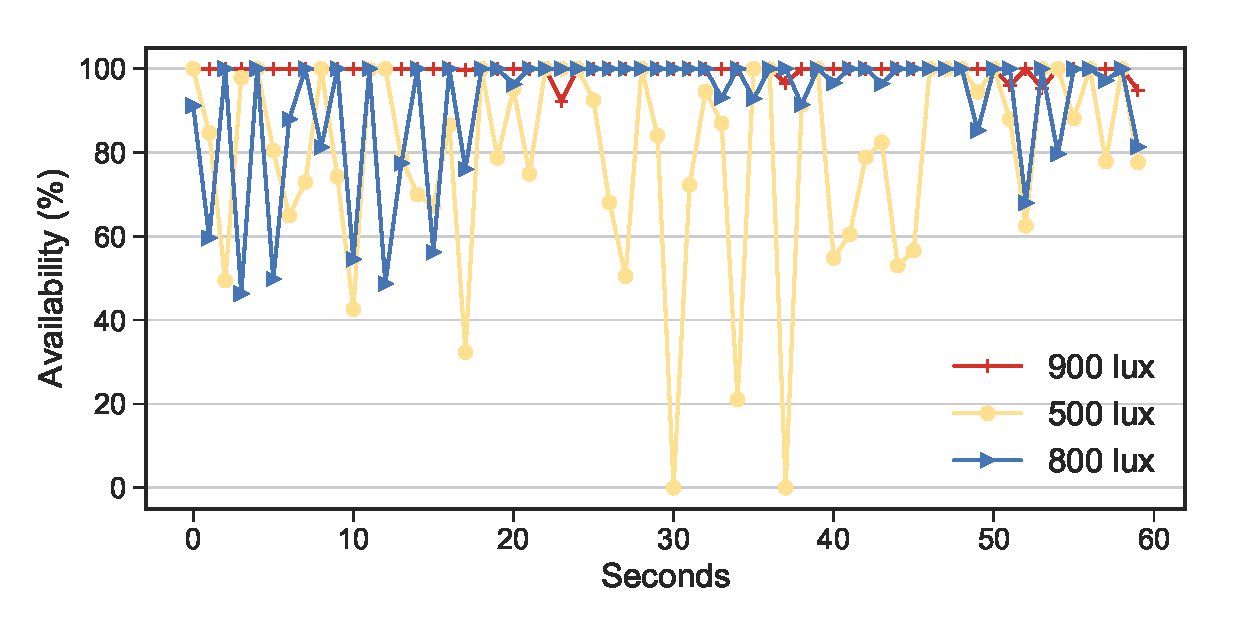
\includegraphics[width=\columnwidth]{figures/sysAvailabilityTimeline_470_sleep_5seconds}
    \caption{\cis availability observed with a 5 seconds time window.}
    \label{fig:fineScaleAvailability}
\end{figure}
% In Section~\ref{subSec:availability}, we discussed that the \cis availability is not a constant value. 
Since the nodes' on-times are in a constant shift relative to each other (Section~\ref{subSec:availability}), the collective availability of the \cis fluctuates when it is observed in a short time window. 
Figure~\ref{fig:fineScaleAvailability} captures \cis availability on a time window of 5 seconds for thee different ambient energy conditions. In these experiments, the average power cycles of the \cis's nodes are (3,18), (3.9,12.3), and (4.3,11.5) seconds when ambient light intensity are 500, 800, and 900\,$\si{lux}$, respectively. 
If we focus on the line graphs associated with 500 and 800\,$\si{lux}$ and compare the system availability within the interval $[20,50]$ seconds and the rest, we can observe that the \cis gradually alternates between low and high collective availability; nodes' on-times gradually transition from maximum to minimum separation and vice versa (Section~\ref{subSec:availability}). Notice that, when ambient light intensity was 800\,$\si{lux}$ the \cis collective availability transited from low to high to low, while this pattern happened to be reversed when light intensity was  500\,$\si{lux}$. For the 900\,$\si{lux}$ the 8-node \cis achieved near-continuous $100\%$ availability. 
%
% \begin{table}
%     \centering
%     \caption{The \cis availability on fine scale: the effect of the energy buffer size and the time interval within a \cis is observed on the system availability}
%     \label{tab:availFineScale}
%     \begin{tabular}{r|l|l|l|r}
%     \hline
%     Intervals (sec) & -    & RF ($47\si{\mu F}$)      & -    & light ($470\si{\mu F}$)  \\ 
%     \hline
%     -             & mean  & std     & mean     & std   \\ \hline
%     0.5             & 61    & 8.8     & 27.3     & 42.9   \\
%     1               & 61    & 5.9     & 27.3     & 41.5   \\
%     2               & 61    & 4.4     & 27.3     & 37.5   \\
%     \hline
%     \end{tabular}
% \end{table}

% Table~\ref{tab:availFineScale} captures the \cis availability on fine scale. An obvious but important observation is that the \cis availability flactuates, see the std columns.    for two different energy buffer sizes. 


% \begin{table}
%     \centering
%     \caption{The \cis availability on fine scale: the effect of the energy buffer size and the time interval within a \cis is observed on the system availability}
%     \label{tab:availFineScale}
%     \begin{tabular}{r|l|l|l|r}
%     \hline
%     Energy Intensity & -    & RF ($47\si{\mu F}$)      & -    & light ($470\si{\mu F}$)  \\ 
%     \hline
%     -             & mean  & std     & mean     & std   \\ \hline
%     high          & 61    & 8.8     & 91.3     & 24.9   \\
%     medium        & 43    & 7.4     & 67.6     & 44.3   \\
%     how           & 21    & 3.4     & 27.3     & 37.5   \\
%     \hline
%     \end{tabular}
% \end{table}




\subsection{Sensing}
\subsubsection{Experiment setup}
\label{sec:experiment_setup}
% \paragraph{availability on a fine scale}
 % \todo{Because of the differences in intermittent nodes power cycles, their duty cycles are constantly shifting relative to each other ( Figure~\ref{fig:cisOntime}).  However, this study does zoom in on the \cis availability on short time scale and the effect of length of the differences between the nodes power cycles on the system short term availability. } 
%
After validating our observation on different energy sources, we designed a testbed with controllable light intensity for clarity and reproducibility. To this end, we blocked uncontrollable light sources with a box of $60 \times 40 \times 40$\,cm. On the box ceiling, we attached a light strip of 2.5\,m with 150 LEDs that can produce 15 different light intensities. On the bottom a \fullCIM of 8 intermittent nodes is placed (see Section~\ref{sec:hardware} for hardware description).

The events in our experiments are spoken words (Table~\ref{tab:words}). 
Short events (see events classification in Section~\ref{sec:event_classification}) are represented with individual words, while burst events are represented with phrases of a few words.
We recorded different patterns of inter-event and inter-bust arriving time. We used a Bluetooth speaker~\cite{jbl} to replay a certain recording. The data were collected using a logic analyzer~\cite{saleae} and processed on a laptop running Ubuntu 16.04 LTS. 
%
\subsubsection{Events detection rate}
%
\begin{figure}[t!]
		\centering
	    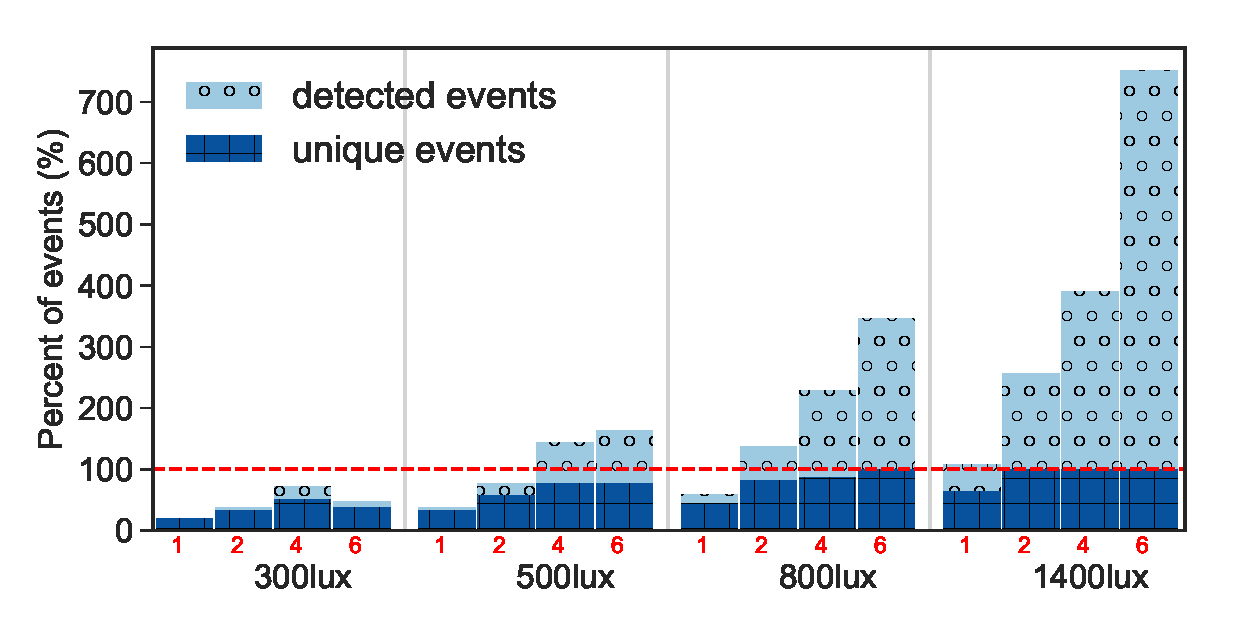
\includegraphics[width=\columnwidth]{figures/regular_events_capture_rate.eps}
		\caption{Duplicate and unique events captured by a \fullcim of eight solar-powered nodes. In general, the number of captured events increases in two case: when light intensity rises and when inter-event arrival time increases. 
         % In general, we see that when the light intensity increases, the number of detected and captured events rise too. Moreover, there is a positive correlation between the length of the inter-event arrival time and the detection and capture rates. 
         Red numbers indicate events arrival interval in seconds.
         }
    	\label{fig:events_detection_rate}
\end{figure} 
Here we experiment with the behavior of a \cis when events arrive individually or in bursts \emph{without} enabling  randomized response in favorable energy conditions. 
%
\begin{figure}[t]
    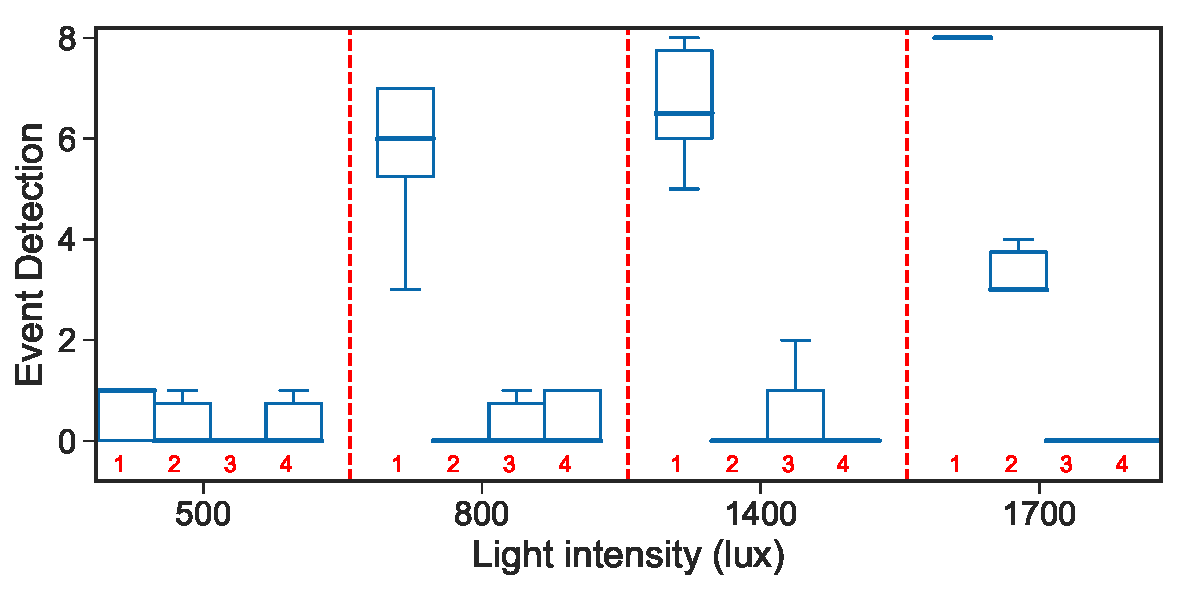
\includegraphics[width=\columnwidth]{figures/events_burst_problem}
	\caption{When capturing a burst of 4 events without randomizing the response, the majority of the nodes react to the first event in the burst and power down shortly after, missing the rest of the burst. Red numbers indicate events index in a burst.}
    \label{fig:events_burst_problem}
\end{figure}
%
\paragraph{Individual events.}
\begin{figure}[t]
	\centering
     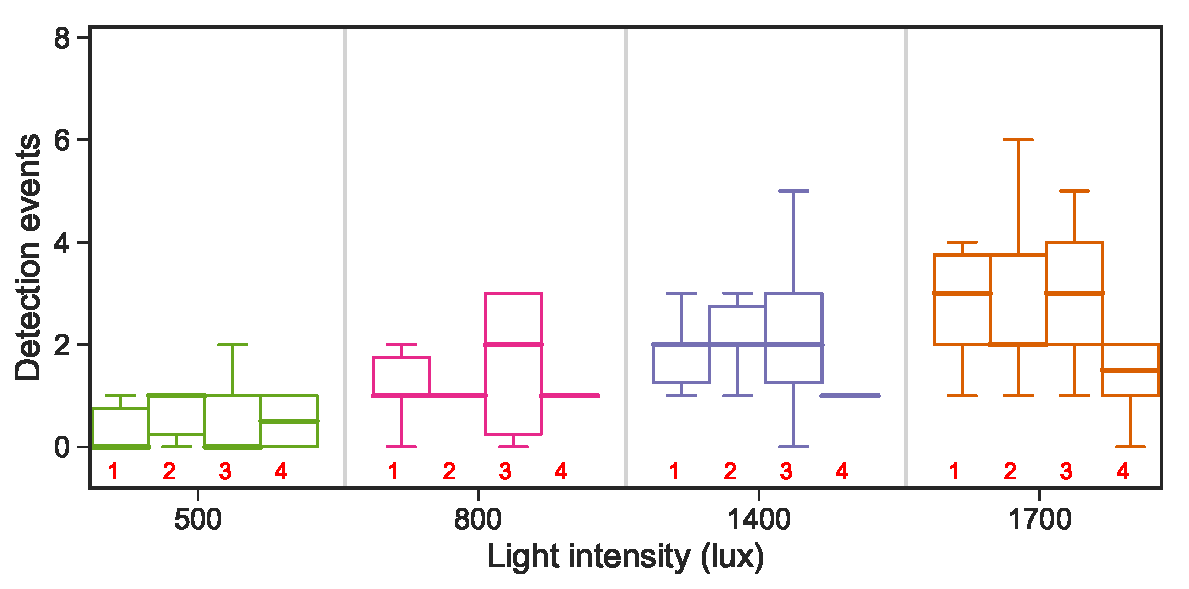
\includegraphics[width=\columnwidth]{figures/events_burst_rand}
    \caption{Response randomization enables a \cis to capture the entire burst of events with high capturing rates. It also reduces the number of duplicated events. Red numbers indicate events index in a burst.}
    \label{fig:events_burst_rand}
\end{figure}

Figure~\ref{fig:events_detection_rate} shows the percentages of capturing duplicate and unique events when light intensity varies from $\SI{300}{lux}$ to $\SI{1400}{lux}$ and the inter-event arrival time ranges from $\SI{1}{sec}$ to $\SI{6}{sec}$. For each experimental trial 20 words were played, resulting in a total of 240 playbacks. 

Figure~\ref{fig:events_detection_rate} clearly shows a positive correlation between light intensity and the number of detected events. In particular, the number of duplicate detections rises dramatically when light intensity increases, \emph{demonstrating the overpowering problem} (Section~\ref{sec:power_state}). Moreover, increasing the inter-event arrival time also surges the number of duplicated events. The reason for this phenomenon is that when the time between events increases, the intermittent nodes get the chance to sleep longer in low-power mode, consuming less energy. Therefore, nodes' on-times expand, reducing their inherent randomization, which leads them to be in \textit{hibernating power state} (Section~\ref{it:hibernating}).  

% Indirectly, these results show how a \cis can achieve a much higher duty cycle than its individual intermittent nodes: Figure~\ref{fig:cis_nodes_dutyCycle} shows that with a light intensity of $\SI{800}{lux}$ an intermittent node is active with a duty cycle of 30\% while Figure~\ref{fig:events_detection_rate} shows that a \cis of 8 nodes captures 100\% of the unique events when the time between them is \SI{6}{s}. 

\paragraph{Bursty events.}
Figure~\ref{fig:events_burst_problem} shows the capturing behavior of a \cis when the events arrive in bursts. A burst of four events with one second between the individual events was fired every 20 seconds. Each burst was repeated 10 times and under four different light intensities. The nodes sleep in a low-power mode when they finish processing an event, waiting for the next one. 

In general, we observe that in favorable energy conditions (above $\SI{500}{lux}$) intermittent nodes react to the first event of a burst and power down shortly after, missing the rest of the burst. These results confirm our argument about the side effect of the \textit{hibernating power state} of a \cis (Section~\ref{sec:power_state}). These results also demonstrate that the hibernating power problem happens on a wide range of power intensities, showing its significance. Next, we will show how randomizing the response can mitigate the problems generated when ambient energy exceeds the design point. 

\subsubsection{Events detection rate with randomization}
\begin{table}
	\centering
    $
    \begin{array}{llll}\hline
     \textbf{(lux,second)} & \textbf{(800,6)} & \textbf{(1400,4)} & \textbf{(1400,6)}\\\hline
    \textit{randomization}    & 205/432 &  236/675 & 223/493 \\
    \textit{no randomization} & 240/831 &  240/938 & 240/1802 \\\hline
    \end{array}
    $
    \caption{These results are presented in the following format \textit{unique/total} detected events. A \cis's node responds with a probability of 65\% in the first two scenarios,\textbf{(800,6)} and \textbf{(1400,4)}, and 30\% for the last one.   
    Randomizing the response reduces the number of duplicated events by 50\% while losing only 7\% of the unique events.}
    \label{tab:regular_rand}
\end{table}
% 
Here, we examine the effect of enabling artificial randomization on the \cis's response. 

\paragraph{Individual events.} 
Table~\ref{tab:regular_rand} compares the number of detected events when the \cim's response is randomized and not randomized.
When randomization is enabled, nodes respond to events with a probability of 65\% for the scenario of $\left(\SI{800}{lux}, \SI{6}{seconds}\right)$ and $\left(\SI{1400}{lux}, \SI{4}{seconds}\right)$, and for the highest energy level and the longest inter-event arrival time the responding probability was set to 30\%.

Table~\ref{tab:regular_rand} shows that randomizing the response reduces duplicated events by an average of $\approx$50\%, while only marginally lowers the number of the uniquely detected events (7\% on average). 

\paragraph{Bursty events.}
To enable a \cis to capture events arrive in bursts, the response probability for each events in a burst should be different. The \cis should respond with a minimum probability to the first event in a burst and gradually increase the response probability for the subsequent events in the burst (we assume that between the bursts the \cis resumes to its expected collective availability). This gradual increment to the responding probability is motivated by the observation that when a node captures an event it becomes unavailable for the subsequent ones in the burst.
In this experiment, the nodes reacted with a probability of 40\%, 50\%, 70\% and, 100\% on the first, second, third and fourth event, respectively. Since the event distribution is known these probabilities were fixed during the development stage.

Figure~\ref{fig:events_burst_rand} shows how randomizing the \cis response spreads the nodes' awake times--as compared to Figure~\ref{fig:events_burst_problem}--and enables the \cis to capture the entire burst with a high probability, i.e., above 85\%. Additionally, we also observe a positive impact of randomizing the response when the system is under-powered ($\SI{500}{lux}$).

%40 50 70 100


% \subsection{Coalesced intermittent command recognizer word detection accuracy}
% For evaluating the \fullcim accuracy, we used the word set in Table~\ref{tab:words}.
% Each word was pronounced by a single speaker 20 times and recorded on a PC. One of these recordings was stored as a template on the \cim, while the remaining 19 were played back through a Bluetooth speaker~\cite{microphone} for testing.

% The ratio between detected events and successfully recognized events per node is shown in Figure~\ref{fig:word_freq} and it averages out at  76.7\%. The difference between detection and capture is primarily caused by nodes that have insufficient buffered energy to finish recording.  

% %
% \begin{figure}
% \centering
% 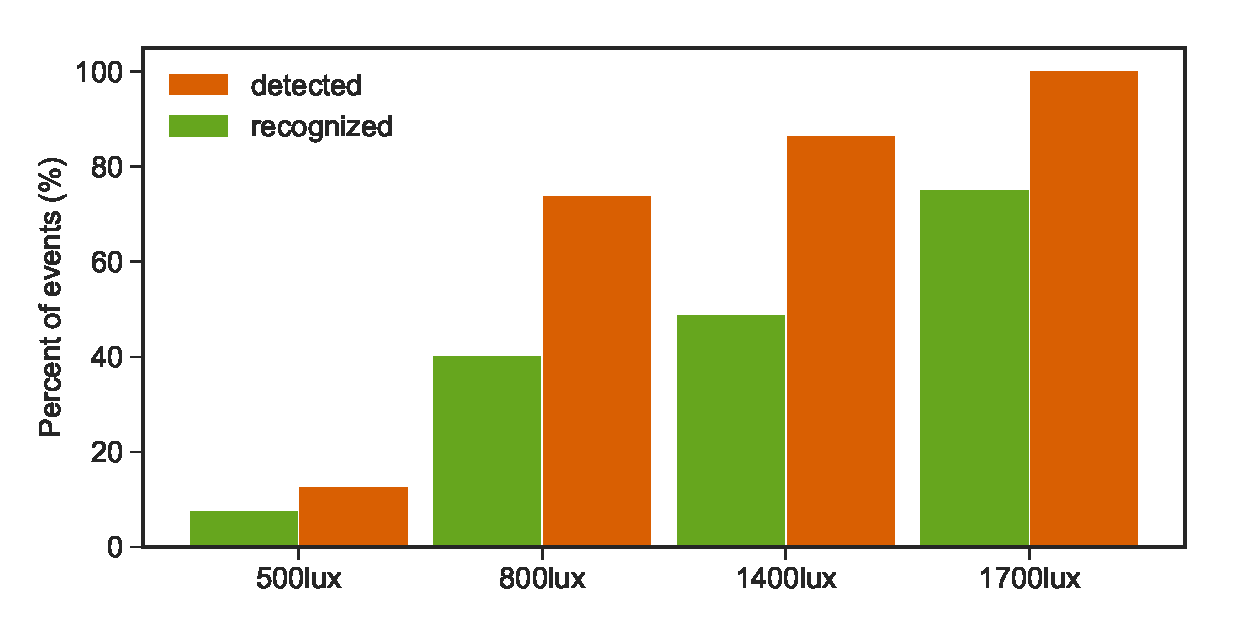
\includegraphics[width=\linewidth]{figures/detection_vs_recognition}
% \caption{
% % The percentage of successfully recognized words as compared to the detected ones.
% The average number of successfully recognized words per node and average number of detected words per node, as percentages of the total number of played words. Words are relatively long events and therefore some of their recordings do not complete due to insufficient harvested energy.}
% \label{fig:word_freq}
% \end{figure}










































